\documentclass[10pt,conference,compsocconf]{IEEEtran}

\usepackage[utf8]{inputenc}
\usepackage[]{algorithm2e}
\usepackage{gensymb}
\usepackage{amssymb}
\usepackage{amsmath}
\usepackage{graphicx}
\usepackage{caption}
\usepackage{subcaption}
\usepackage{wrapfig}
\usepackage{url}
\usepackage{hyperref}
\usepackage{float}
\usepackage{xcolor}
\usepackage{listings}


\begin{document}

\title{A Directional Diffusion Algorithm for Inpainting}

\author{
  Team \textit{MassiveGainz}\\Jan Deriu, Rolf Jagerman, Kai-En Tsay\\
  Department of Computer Science, ETH Zürich, Switzerland
}

\maketitle

\begin{abstract}
The problem of inpainting involves reconstructing the missing areas of an image. Inpainting has many applications, such as reconstructing old damage photographs or removing obfuscations from images.
In this paper we present the directional diffusion algorithm for inpainting. Typical diffusion algorithms are bad at propagating edges from the image into the unknown masked regions. The directional diffusion algorithm improves on the regular diffusion algorithm by reconstructing edges more accurately. It scores slightly better than regular diffusion when reconstructing images that are obfuscated by a text mask. 
\end{abstract}

\section{Introduction}
\label{sec:introduction}

Automatically filling in missing areas of an image is an inference task often referred to as inpainting. It is commonly used to restore old damaged photographs or to remove small objects from an image \cite{bertalmio2000image}. These two settings are inherently different. The first needs to restore many small areas of an image. The second restores a few large areas of an image.

In this paper we introduce a novel approach that solves the inpainting task for the first setting, restoring small damaged areas in pictures. Our approach is based on the diffusion algorithm described by McKenna et al. \cite{richard2001fast}.

The paper is structured in several sections. First we will describe the methods we use to accomplish the inpainting task in section \ref{sec:methods}. Next we will discuss the results of our methods in section \ref{sec:results} and compare them to several baselines. In section \ref{sec:discussion} the strengths and weaknesses of our novel approach are discussed. Finally the paper is concluded in section \ref{sec:conclusion} and possible future work is described in section \ref{sec:futurework}.


\section{Methods}
\label{sec:methods}

We present two algorithms that accomplish the inpainting task: regular diffusion and directional diffusion. The first is a naive yet fast approach. The second is an extension of the first, which takes into account the directionality of image patches to perform smarter diffusions. Although it is slower, it typically leads to better results.

\subsection{Regular diffusion}
The idea of diffusion is to fix the known regions of the image and let them diffuse into the unknown regions. This can be done very efficiently by using a convolutional kernel. By iteratively convolving a kernel with the entire image and then restoring the known pixels we can obtain an inpainted image. This process is described in algorithm \ref{alg:diffusion}. The quality of the solution heavily depends on the kernel used. A variety of kernels can be used, two of which are displayed in figure \ref{fig:kernels}. To convolve a kernel with an image we have to refer to pixels outside of the border of the image. We replicate the borders of the image outwards so the kernel can properly refer to these values.

\begin{figure}
\begin{flalign*}
K_{\text{diamond}} &= \begin{bmatrix}0 & 0.25 & 0 \\ 0.25 & 0 & 0.25 \\ 0 & 0.25 & 0\end{bmatrix}\\
%K_{\text{gauss}} &= \begin{bmatrix}0.011 & 0.084 & 0.011\\0.084 & 0.620 & 0.084 \\0.011 & 0.084 & 0.011\end{bmatrix}\\
K_{\text{diag}} &= \begin{bmatrix}0.38 & 0.04 & 0.04 \\ 0.04 & 0 & 0.04 \\ 0.04 & 0.04 & 0.38\end{bmatrix}
\end{flalign*}
\caption{Kernels used for diffusion.}
\label{fig:kernels}
\end{figure}

\begin{algorithm}
	\KwIn{Image $I$, mask $M$, kernel $K$ and threshold $\epsilon$}
	\KwResult{Reconstructed image $I_{r}$}
	$K \leftarrow \frac{K}{\sum_i \sum_j K_{i,j}}$ (normalize $K$ to preserve energy)\; 
	$I_{prev} \leftarrow 0_{size(I)}$\;
	$I_{r} \leftarrow I$\;
	\While{$\|I_{r} - I_{prev} \|_{F} > \epsilon$}{
		$I_{prev} \leftarrow I_{r}$\;
		$I_{r} \leftarrow \text{convolve}(I_{r}, K)$\;
		$I_{r} \leftarrow I_{r} \circ \mathbf{1}_{M = 0} + I \circ \mathbf{1}_{M \neq 0}$ \;
	}
	\quad
\caption{Diffusion algorithm for inpainting. We denote element-wise multiplication with the $\circ$ operator. The $\mathbf{1}_{M=0}$ function represents a matrix with elements $(i,j)$ set to 1 when $M_{i,j}=0$ and 0 otherwise.}
\label{alg:diffusion}
\end{algorithm}
\begin{figure}
	\centering
	\begin{subfigure}[b]{0.4\textwidth}
		\centering
		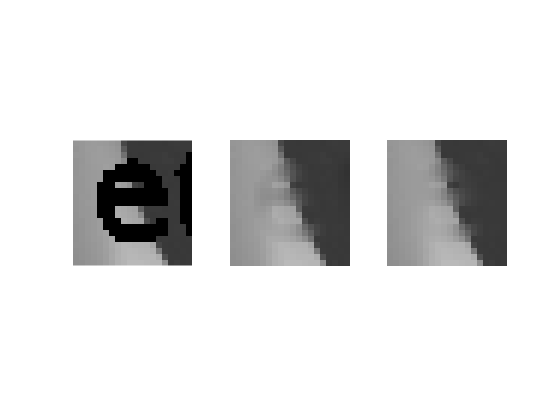
\includegraphics[clip, trim=0cm 5.2cm 0cm 4cm, width=0.85\textwidth]{figures/step-by-step-cross}
		\caption{Diamond kernel $K_{\text{diamond}}$}
		\label{fig:stepbystepcross}
	\end{subfigure}
	\begin{subfigure}[b]{0.4\textwidth}
		\centering
		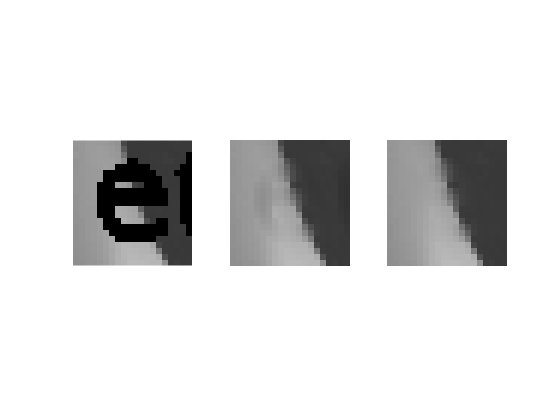
\includegraphics[clip, trim=0cm 5.2cm 0cm 4cm, width=0.85\textwidth]{figures/step-by-step-directional}
		\caption{Directional kernel $K_\theta$ for $\theta = 100\degree$.}
		\label{fig:stepbystepdir}
	\end{subfigure}
	\caption{Step-by-step illustration of the diffusion process with different kernels. Each step represent 20 iterations.}
\end{figure}

\subsection{Directional diffusion}



\section{Results}



\section{Discussion}
\label{sec:discussion}

\begin{figure*}
	\centering
	\begin{subfigure}[b]{0.49\textwidth}
		\centering
		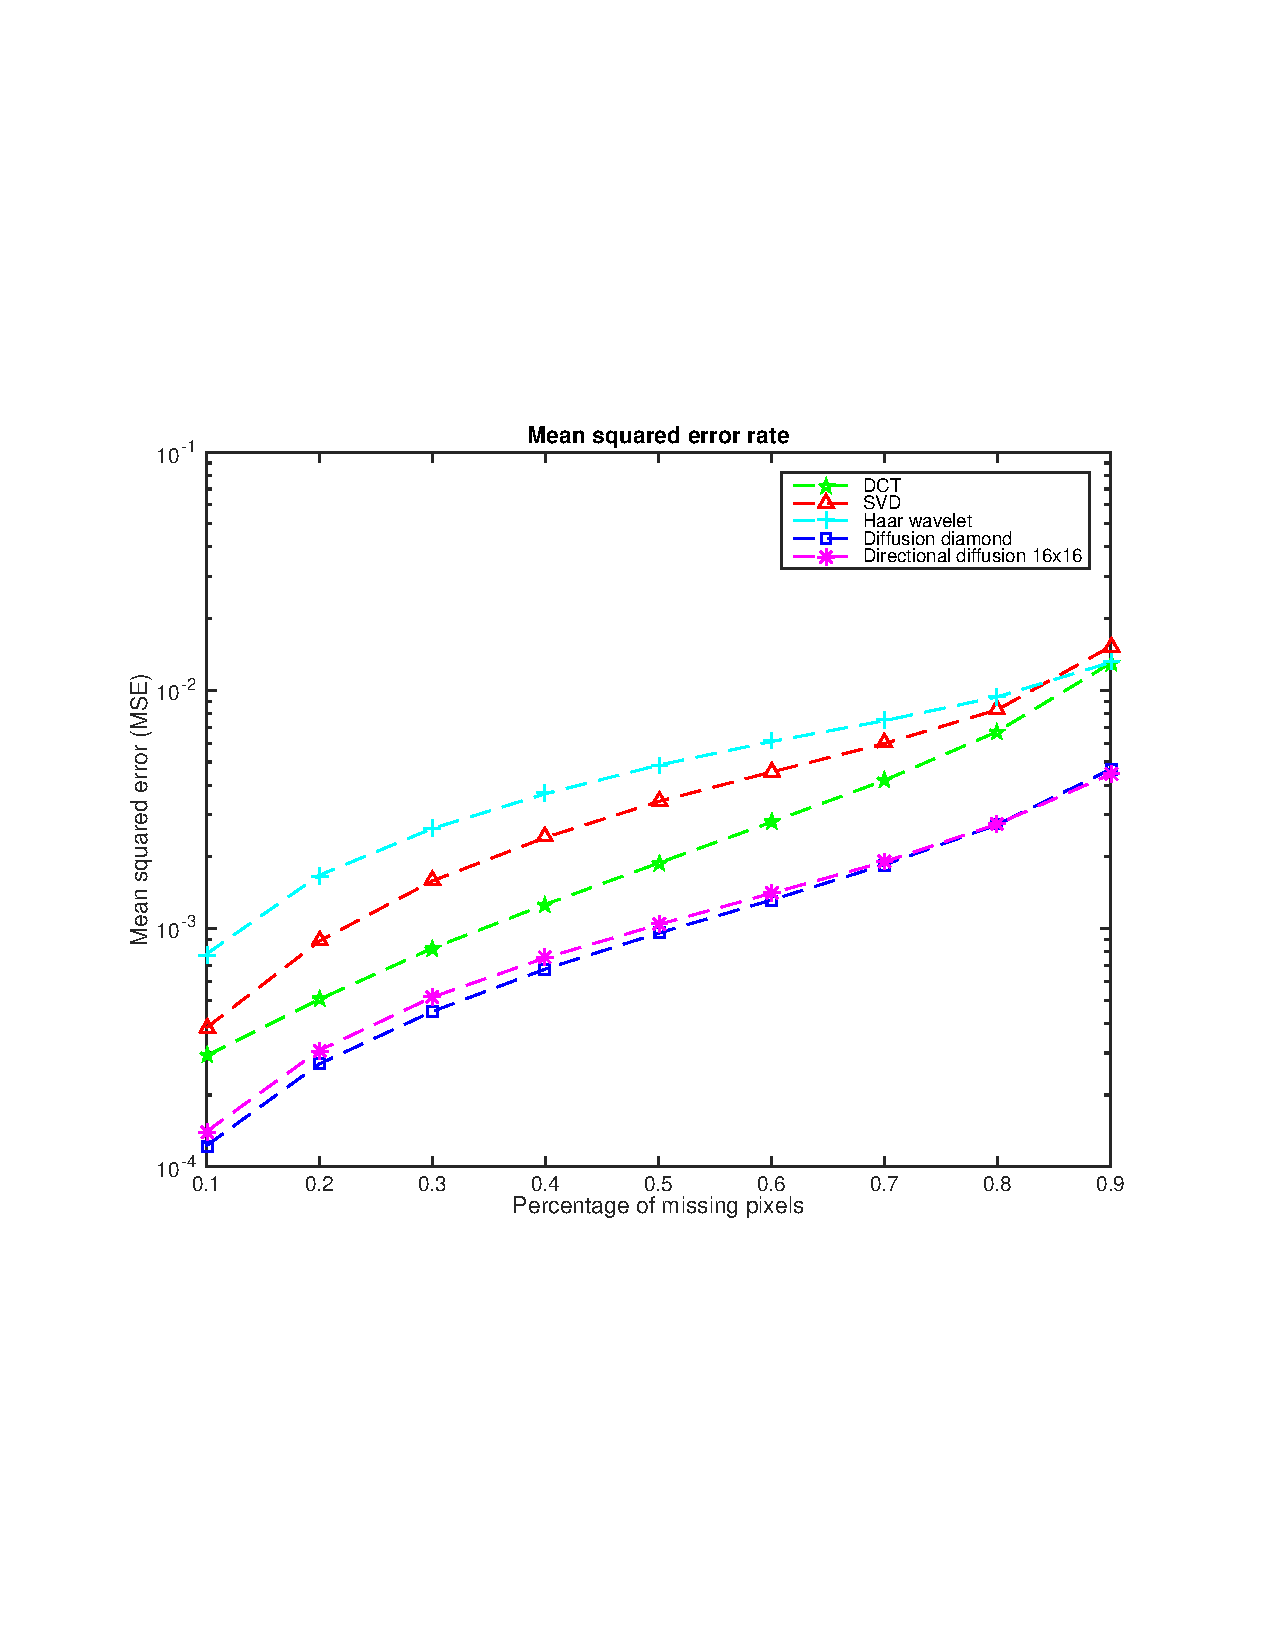
\includegraphics[clip, trim=2cm 7cm 2cm 6cm, width=0.9\textwidth]{figures/mse_vector}
		\caption{Mean squared error in log scale}
		\label{fig:err_random}
	\end{subfigure}
	\begin{subfigure}[b]{0.49\textwidth}
		\centering
		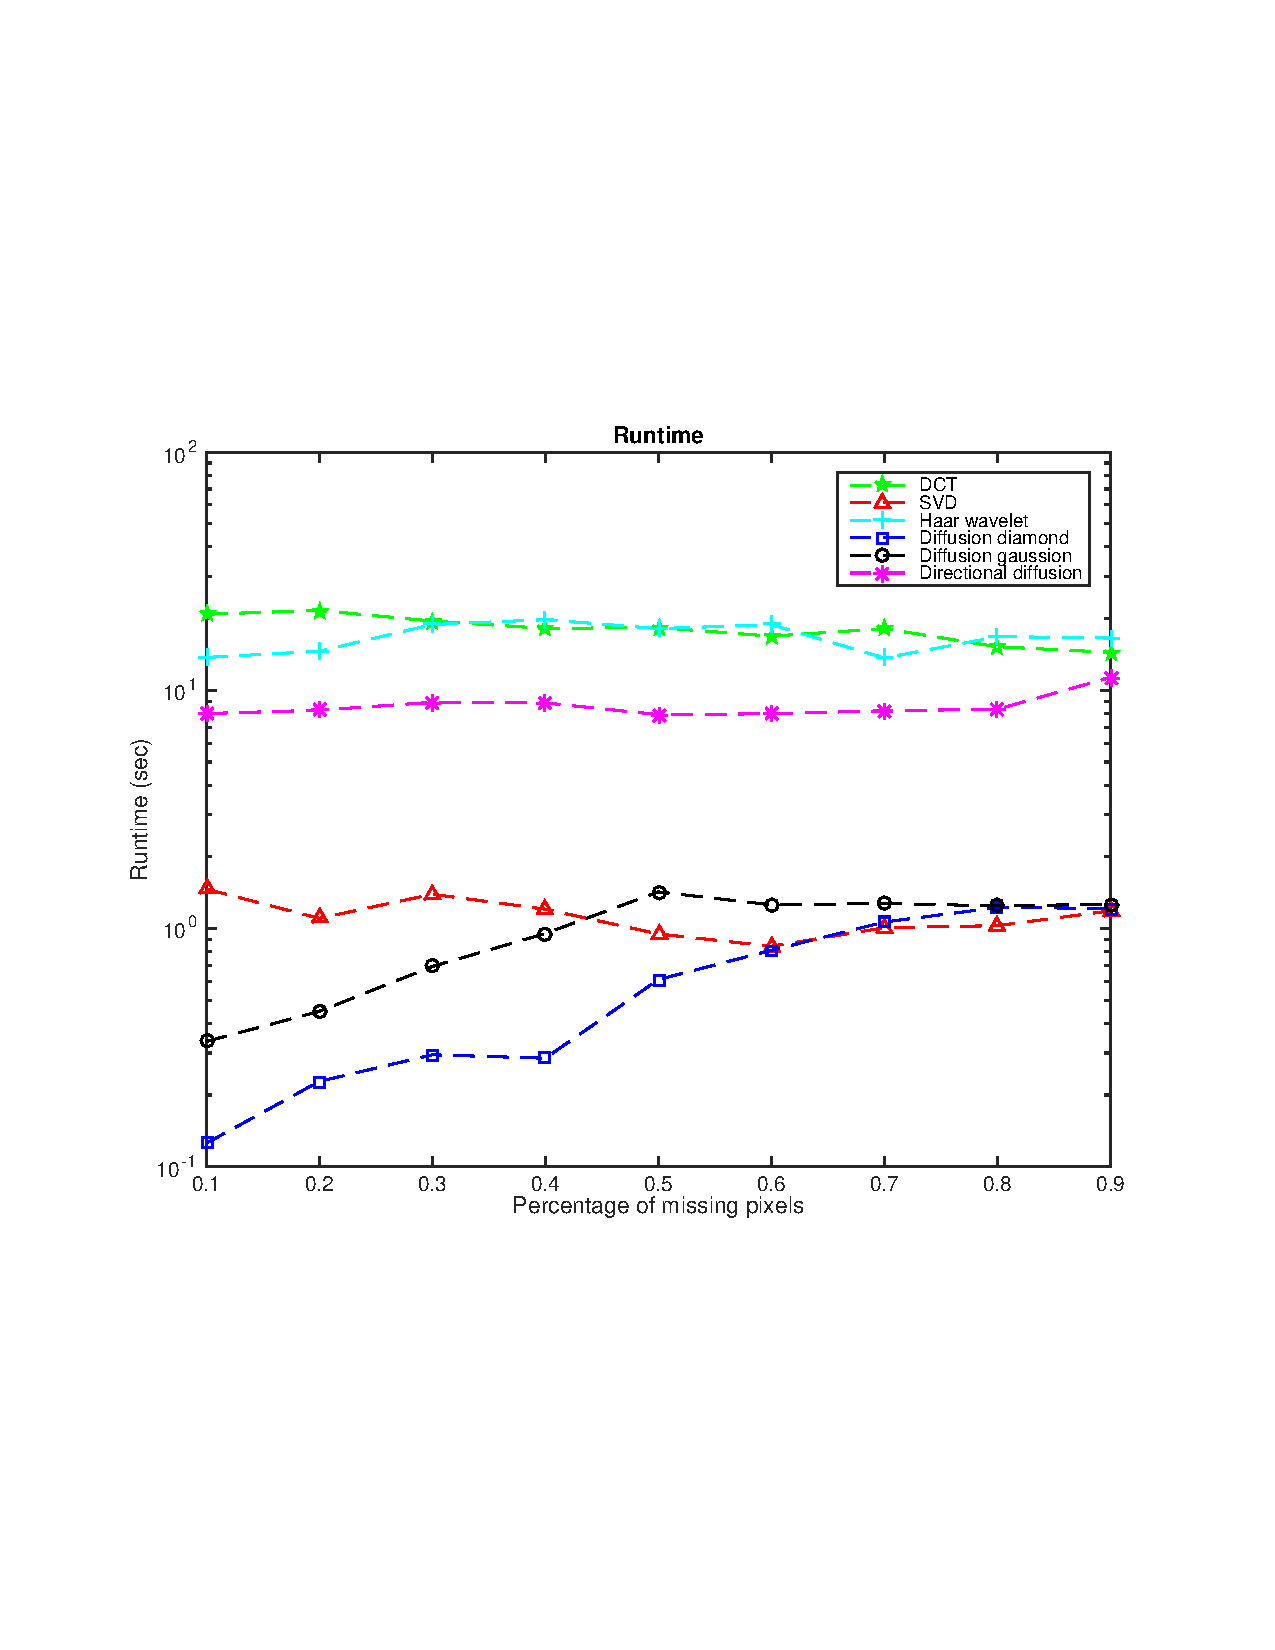
\includegraphics[clip, trim=2cm 7cm 2cm 6cm, width=0.9\textwidth]{figures/runtime_vector}
		\caption{Runtime in log scale}
		\label{fig:runtime}
	\end{subfigure}
	
	\caption{Mean squared error and runtime comparison with different algorithms}
	\label{fig:results}
\end{figure*}


Both the regular diffusion and the directional diffusion algorithm show promising results. From figure \ref{fig:err_random} we see that the regular diffusion algorithm with the $K_{\text{diamond}}$ kernel works best on a mask of randomly missing pixels. This phenomenon can be explained by the fact that this algorithm diffuses nearby pixels into the missing regions. A mask with randomly missing pixels will, on average, have at least some pixels in the direct or near neighborhood of a pixel that we try to inpaint.


Table \ref{tbl:err_text} shows the mean squared error of the algorithms on a fixed mask, namely a piece of text. In this case, the missing pixels have some structure and form medium-sized areas of missing pixels. In that case, the directional diffusion algorithm performs best. As the size of the regions of missing pixels gets larger, the regular diffusion algorithm has less nearby pixels to work with. Any high-contrasting edges of the underlying image are not properly extended into the unknown regions. The directional diffusion algorithms helps resolve this by aligning the kernel  $K_{\theta}$ with the general directionality of the image patch. This attempts to propagate high-contrast edges of the image into the unknown regions. This does however come at the cost of a significant increase in runtime.

Although the directional diffusion scores slightly better than the regular diffusion algorithm on text masks, we feel the trade-off in execution time is not worth the increase in score. Hence we decided to submit the regular diffusion algorithm as a final submission to the scoreboard. In scenarios where the runtime is not a deciding factor, we would select the directional diffusion algorithm due to its lower mean-squared error.

\section{Conclusion}
\label{sec:conclusion}




\section{Future work}




\bibliographystyle{IEEEtran}
\bibliography{cil_report}

\end{document}
